% Ingenieurpraxis
\def\mytitle{realtime FoG detection and hardware implementation}
\def\mykeywords{Freezing of gait, realtime, gait features, lda, DAPHNET}
\def\myauthor{Wei Zhaoxiong}
\def\contact{ge25zir@mytum.de}

\documentclass[article]{article}

\usepackage[a4paper,outer=1.5cm,inner=1.5cm,top=1.75cm,bottom=1.5cm]{geometry}
\twocolumn
\usepackage[utf8]{inputenc}     % Zeichenkodiezrung UTF-8
\usepackage[english]{babel}     % Deutsche Sprache und Silbentrennung
\usepackage{graphicx}           % Bilder
\usepackage[colorlinks,linkcolor={black},citecolor={blue!80!black},urlcolor={blue!80!black}]{hyperref}
\usepackage[parfill]{parskip}   % Stop indentation on new paragraphs
\usepackage{watermark}          % 
\usepackage{lipsum}             % Blindtext
\usepackage{xcolor}             %
\usepackage{listings}           %
\usepackage{float}              %
\usepackage{titlesec}           % 
\usepackage{amsmath}            % Formeln
\usepackage{algorithm2e}        % PseudoCode
\usepackage{caption}
\usepackage{subcaption}
\captionsetup[figure]{font=footnotesize}

\renewcommand*\familydefault{\sfdefault}
\graphicspath{{./img/}}
\hypersetup{pdfauthor=\myauthor,pdftitle=\mytitle,pdfkeywords=\mykeywords}

\titlespacing{\subsection}{0pt}{\parskip}{-3pt}
\titlespacing{\subsubsection}{0pt}{\parskip}{-\parskip}
\titlespacing{\paragraph}{0pt}{\parskip}{\parskip}
\newcommand{\figuremacro}[5]{
    \begin{figure}[#1]
        \centering
        \includegraphics[width=#5\columnwidth]{#2}
        \caption[#3]{\textbf{#3}#4}
        \label{fig:#2}
    \end{figure}
}

\lstset{
	escapeinside={/*@}{@*/}, language=C++,
	basicstyle=\fontsize{8.5}{12}\selectfont,
	numbers=left,numbersep=2pt,xleftmargin=2pt,frame=tb,
    columns=fullflexible,showstringspaces=false,tabsize=4,
    keepspaces=true,showtabs=false,showspaces=false,
    backgroundcolor=\color{white}, morekeywords={inline,public,
    class,private,protected,struct},captionpos=t,lineskip=-0.4em,
	aboveskip=10pt, extendedchars=true, breaklines=true,
	prebreak = \raisebox{0ex}[0ex][0ex]{\ensuremath{\hookleftarrow}},
	keywordstyle=\color[rgb]{0,0,1},
	commentstyle=\color[rgb]{0.133,0.545,0.133},
	stringstyle=\color[rgb]{0.627,0.126,0.941}
}

\thiswatermark{\centering \put(470.0,-20.0){
\includegraphics[scale=0.5]{tum}} \put(0.0,-20.0){
\includegraphics[scale=0.25]{ldv}}}


\title{Ingenieurpraxis\\\mytitle}
\author{\myauthor\hspace{1em}\\\contact\\Technische Universität München}
\date{\today}
\sloppy


\begin{document}
\maketitle

% ABSTRACT
\begin{abstract}
    Freezing of gait(FoG) is an abnormal gait pattern that accompany Parkinson's disease(PD). During such short, temporary periods, the patient is not able to move the feet forward despite the intention of walk. According to the research, a sequence of rhythmic stimuli is able to help patient to walk again during FoG. Therefore, it is important to detect FoG pattern at the very beginning or even before it comes.
    
    In this paper, we tried to extract and select gait features using DAPHNET dataset. A fisher discrimination analysis and feature thresholding is applied to further reduce its dimension. At the end, we proposed a new evaluation standard that focus on improving the user experience.
    
\end{abstract}  
\textbf{Keywords -- }{\mykeywords}

% Introduction
\section{Introduction}
    Parkinson's disease(PD) is the second most common aging-associated neurodegenerative disorder. It is characterized by motor features such as muscular stiffness, resting tremor, hastening of the gait(festination) and poor postural stability. Freezing of gait(FoG) is one of the symptoms of PD, during such sudden and short episode, the patient experiences gait disturbance ranging from complete sudden akinesia to milder leg trembling or short shuffling steps events, usually described by patients as feeling the feet stuck to the floor. However,there is still no effective treatment or drug-resistant against such disease.
    
    The work of XXX shows rhythmic auditory stimulation(RAS) was shown to be particularly effective at improving gait among PD patients. In their experiment, regular metronome ticking sounds were applied as RAS with a rate of 110\% compared to the natural walking rate of tested patient.
 	This served to improve gait stability and speed.
 	
 	Since listening the ticking sounds all time is something quite annoying, a realtime detection of FoG becomes quite important. 
 	
 	  
 	A variety of methods have been presented to detect FoG. Moore et al. used an Inertial Measurement Unit(IMU) mounted around a shank, and defined a freeze index(FI) using power spectrum analysis of accelerometer signals. Each patient use individually calibrated thresholds to recognize FoG. 
 	
 	Based on this, Bachlin et al proposed a real-time FoG detection algorithm combines the FI with a second power threshold to discriminate FoG from normal gait.
 	
 	Rezvanian and Lockhart employed continuous wavelet transform(CWT) on one accelerometer to define an index for identifying FoG. 
   
    Besides, there are also several machine learning based approaches that exploiting the data set. Florenc et al. applied kernel-lda to the accelerometers' raw data to reduce the dimension of features. Then a k-nearest neighbor algorithm(k-NN) was used to classify gait in pre-FoG, no-FoG and FoG. 
    
    The work of Natasa et al. extract features from raw data and using Boruta algorithm to reduce the dimension, they also make a comparison of result using classifiers like Support Vector Machine, Random Forest and k-NN.
    
    Parisa et al. collected  inertia and physiological signals to extract freezing patterns, the set of features are fed into a Fully-Connected-Neural Network(FCNN) to learn and predict freezing episodes.
    
    Considering that some method is too expensive for wearable devices, such as parameters of FCNN takes too much memory space and computational resources and it may hard to meet the requirement of real-time. We are not going to consider it as an option in our setup.

 
    
% Approaches tries
\section{Approaches Pursued}

 	In this research, the data set from DAPHNET Freezing of Gait dataset is used. This dataset consists of sensor data extracted from individuals with PD. Three tri-axial accelerometers were placed at the shank(just above the ankle), thigh(just above knee) and lower back to collect acceleration in three axes with a sample rate of 64Hz.

	The dataset include data from 10 patients, they are asked to perform walking in straight line, walking with numerous turns and some daily living tasks. The label is done by two physiotherapists using video recording.


    In the first part of this research internship, I tried to implement the algorithm of Florenc. However, I failed to separate classes in the test set by using kernel-lda. Also, the author informs that his work does not perform well when it comes to larger data set. So I tried to pursue other algorithms.
    
    Another machine learning algorithm I tried is Neural Network(NN), however, with limited number of weights and layers allowed, it's hard to do the classification correctly.
    
    According to my observation, the reason for the failure employing data-driven methods could be the followings. First of all, the data set is not quite balanced, the FoG labeled data is far less than non-FoG data set. Second, there might be some miss-labeled data. Since the data set is labeled with eye observation, it is possible the detection of FoG is slower than it should have been for second. 
    
    Therefore, most machine learning methods that make the classification generally performs not well.
    
    After a conversation with my advisor, I change the research target to gait cycle analysis. This is a study that is used to assess and treat individuals with conditions affecting their ability to walk. From the data set, it is possible to extract features like walking speed and cadence. After some gait features are extracted, thresholds and machine learning techniques are applied. The general procedure of this method is shown in figure 1. More detail information can be found in next section.
    
    
    \begin{figure}
    	\centering
    	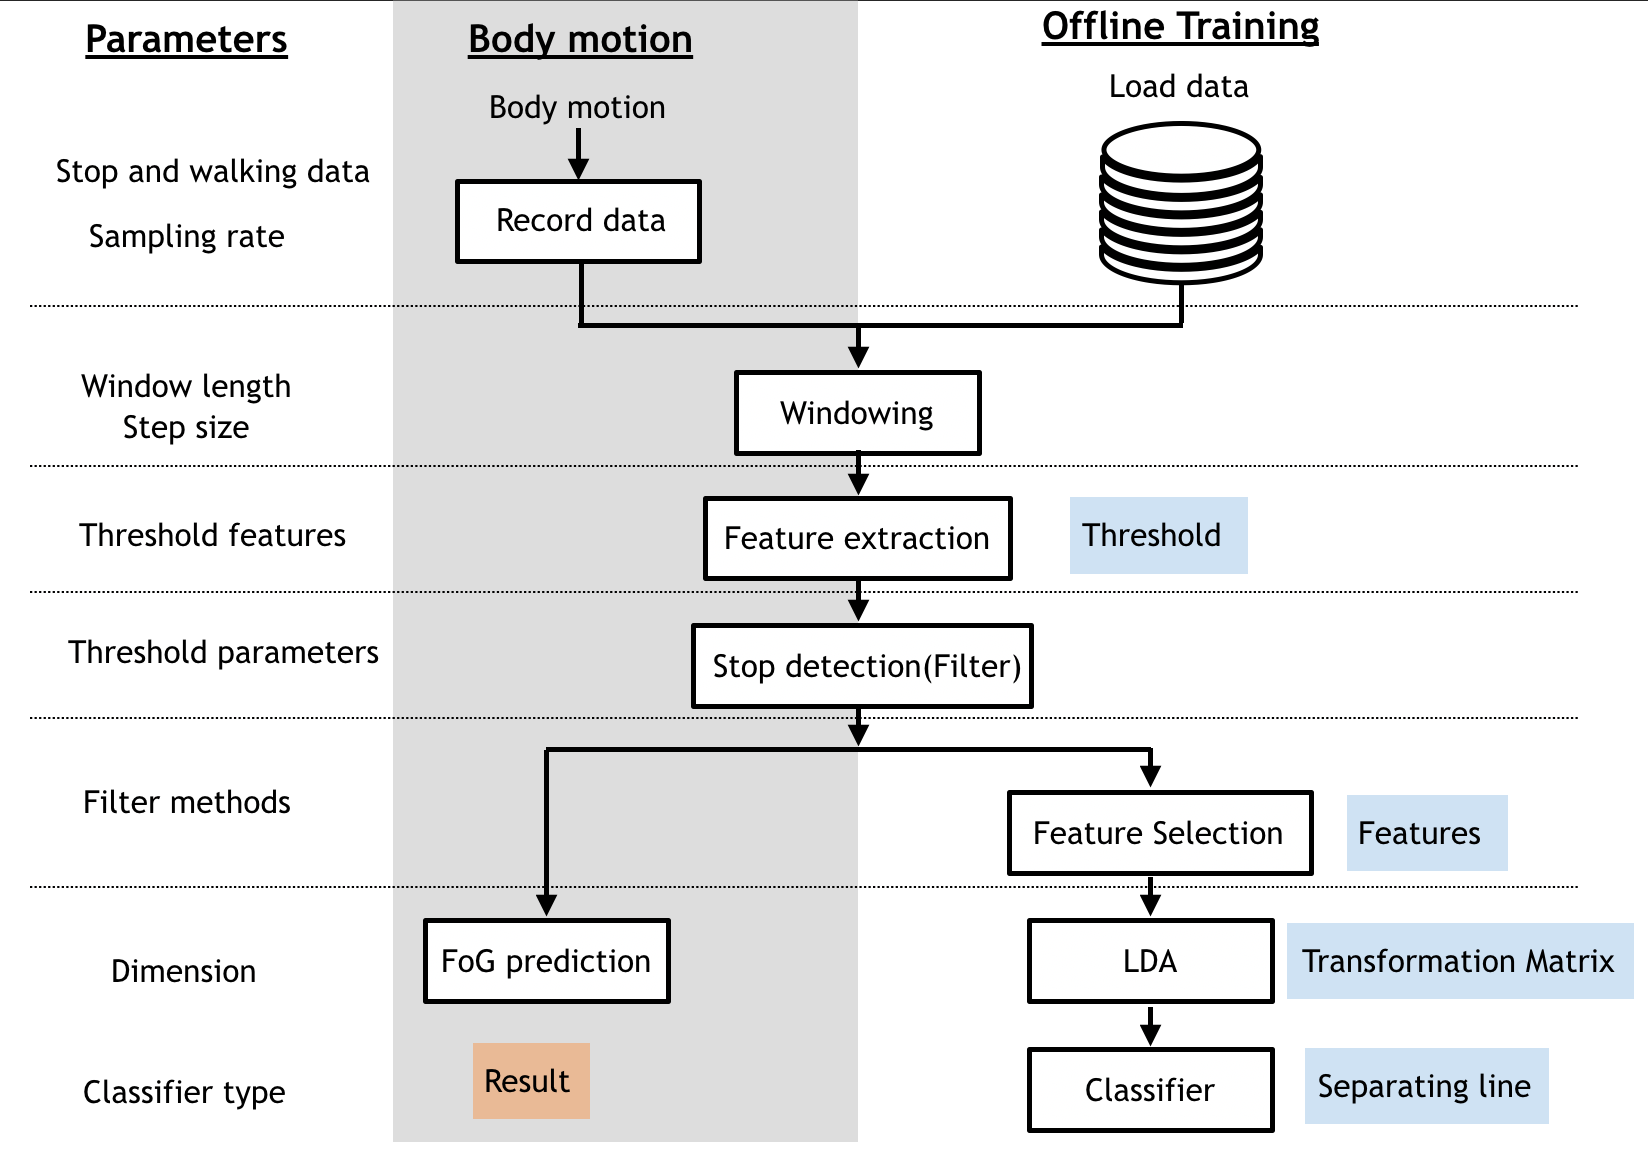
\includegraphics[width=0.47\textwidth]{procedures}
    	\caption{}
    	\label{fig:y equals x}
    	
    \end{figure}
% Method
\section{Method}
    Some methods used thresholds on several important features directly to filter out FoG period, while the others applied machine learning methods to extract features and do classification.

In the proposed method, we are trying to combine these two
method together.

According to previous experience, it is hard to use LDA or PCA directly on raw data or low-pass filtered data to extract features with generality because of the unbalanced data and noises.
However, simple gait feature extraction followed by thresholds and LDA do not yield good result either. More pre-processing work need to be done to further reduce the influence of noise. 

It is important that this filter only does some coarse filtering and does no break the FoG in training data into small pieces. 


Then a feature selection procedure is done to further reduce the dimension of features and reduce noise from uncorrelated features.

The first procedure added is called pre filtering. Before the LDA, features like total energy in the gait window can filter out gaits for walking, turning and FoG. The dataset is more balanced after this step.

In the next step,  we use feature selection methods based on correlation or mutual information to filter away features on different channels that are not efficient. Since the FoG feature do not express itself equally on all axis. Also, different patient has different reactions during FoG.  

After the feature dimension is reduced, LDA is applied to remained good features to reduce the dimension, followed by SVM, random forest and other machine learning classification methods. The result of classifier can further get filtered with other filters to get a final result.  

\subsection{Data Preprocessing}

	The sliding window is choosed as 2 seconds with 256 * 9 floats per window. The step length is chosen as 0.5 seconds. It is also possible to try longer window length, the influence is not going to be discussed here.
	
	As mentioned before, there is a huge unbalance between FoG labeled and non-FoG labeled data. Also, we would like to detect FoG as soon as possible, so for each window before a FoG window, we also label it as FoG window, this reduce the number of non-FoG window and increases FoG windows. 
	
	

    

% Features Extraction

\subsection{Feature extraction}


	The features can be extract from both time domain and frequency domain. 
	
	From the observation of acceleration data in time domain, we can visualize clear some periodic pattern during the non-FoG phase, However, such characteristic is less obvious or not existing in FoG phase.The following three methods can be applied to exploit such observation.

	\begin{enumerate}
		\item Sample Entropy: A measure of complexity, Often used to analyze the physiological variability in human gait and it is derived from approaches developed by Richman and Moorman. A feature which shows the repeatability and predictability within one window. The formula used to calculate it is:
    
		    \begin{equation}
		        \mathbf{SampEn} = -log A/B
		    \end{equation}
   
		   In this study the dimension m is selected as 2, r = 0.2*$\mathbf{\delta}$ 
  
		
	\item Cross Correlation :Another method to exploit the periodicity is to use cross correlation. This shows the similarity between a signal and its shifted version. The window size in our case is selected as 2 seconds, so generally 2 to 3 steps can be observed in it. In this way,a shift with highest value can be considered as a step interval.
		
		\begin{equation}
		\mathbf{CrossCorrelation} = \sum_{n=0}^{n=len} f[n]g[n+\delta]
		\end{equation}
		
		Besides, the highest correlation value also shows the possibility of existing a periodic pattern in this window, which can be used as another feature.
		
		


	\item Fast step detection: Both methods mentioned before is quite expensive in terms of time, and when it is implemented on hardware the realtime capability might not be guaranteed. 
		
		Therefore, we invented a more light-weight method based on the observation from data. A step usually comes with a large drop and rise in the acceleration data, such U shape can be used as a feature to detect one step. As the figure shows, we can search for continuous decrease in the value and find potential step points. With such information we can find the step interval, step frequency.
		
		The result is as the figure 1 shows, between 50 and 250 we can clearly see the patient is walking normally, so the step interval most of time stays at 60ms. Whenever the patient turns, we can clearly observe some gap. When the patient experience FoG, the step interval can decrease to 0 for patient 2.	

	\end{enumerate}


	


	From another point of view, we can also extract useful information from frequency domain.
	
	 
	 The information could be extract with two methods
	 
	\begin{enumerate}
		\item Dominant frequency peak: Dominant frequency is defined as the highest magnitude frequency in a power spectral density. This is the frequency which carries the most energy. Generally speaking, this value should coincide with step speed of walking during normal walking, which is 1-2 Hz. 
	
		\item Freezing Index and energy thresholds: Moore et al. discovers that more energy components appears
			in [3-8Hz] band during FoG. They introduced a freeze Index(FI) as a strong indicator of FoG.
			
			To calculate FI, we apply a method proposed by Baechelin et al., they used a 256-point FFT to get power spectral density. The locomotion energy is calculated as the integral in [0-3Hz], and freeze energy is integrated in [3-8Hz]. The freeze Index is calculated as :
			\begin{equation}
			\mathbf{FI} = loco/(loco+freeze)
			\end{equation}			
			
			Furthermore, according to the measurement of Baechelin et al. The total energy content in band [3-8Hz] of standing is significantly lower than that for FoG and for walking. This feature can be employed to filter out windows that patient is not moving.
			  

	
		\item Wavelet mean: Wavelet transform is a standard tool that shows how the power amplitude of a specific frequency in a signal change over time. In the paper of Rezvanian and Lockhart et al., they used the ratio of sum of wavelet coefficient in freeze and locomotion bands to discriminate FoG and non-FoG events. Here we used the mean of absolutes values of Discrete Wavelet Transform(DWT) from level three which includes freeze band. Daubechies wavelet of order four is chosen as mother wavelet. 
	
	\end{enumerate} 
\begin{center}
	\begin{table}
	\begin{tabular}{ |p{2cm}||p{6cm}|  }
		\hline
		\multicolumn{2}{|c|}{Features in time domain} \\
		\hline
		Features & Description\\
		\hline
		sample entropy & Measures repeatability or predictability within one window : \\
		\hline
		step interval & Time interval between two steps in one window\\
		\hline
		max correlation & Measures the periodicity in one window\\
		\hline
		step depth & Difference between max and min value in one window\\
		\hline
		step counts & Counts of steps in one window \\
		\hline
		variogram & The measure of smoothness of data in time series \\
		\hline
		portion above mean &The proportion above the mean of the observationswithin the window whose values are greater than
		the mean of the window \\
		
		\hline
		\multicolumn{2}{|c|}{Features in frequency domain}
		\\
		\hline
		Features & Description\\
		\hline
		loco-band energy & energy in [0.5-3Hz] frequency band\\
		\hline
		loco-band+freeze-band energy & energy in [0-8Hz] frequency band \\
		\hline
		freezing index & The power in the 3-8Hz band divided by the power in 0.5–3 Hz band  \\
		\hline
		dominant frequency & The frequency with maximal Power Spectral Density (PSD) \\
		\hline
		wavelet mean & the mean of coefficient of DWT in the third level, which represents energy in freeze band \\
		
		\hline
	\end{tabular}
\caption{Features}
\end{table}
\end{center}

\begin{figure*}
	
	
	\begin{subfigure}[b]{0.47\textwidth}
		\centering
		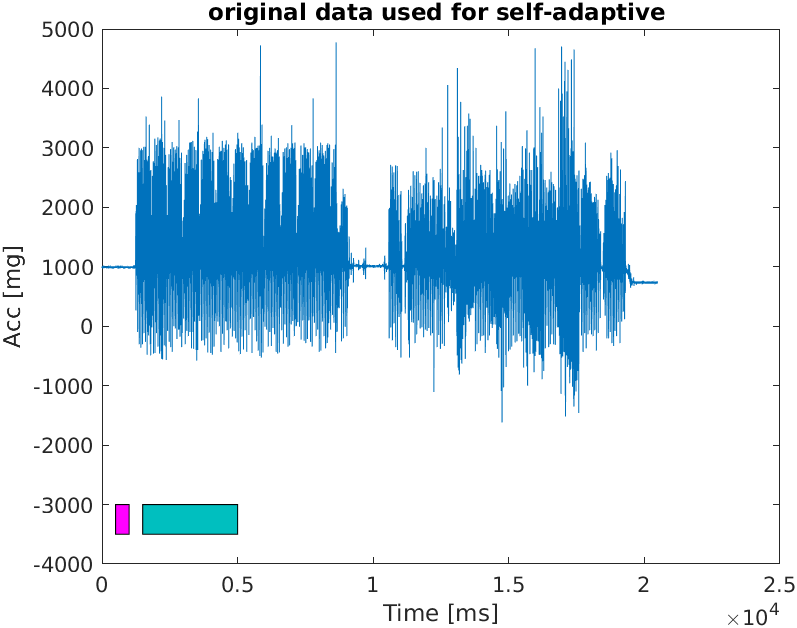
\includegraphics[width=\textwidth]{training_data_s2_p2}
		\caption{acceleration in x axis of ankle sensor}
		\label{fig:y equals x}
	\end{subfigure}
	\hfill
	\begin{subfigure}[b]{0.47\textwidth}
		\centering
		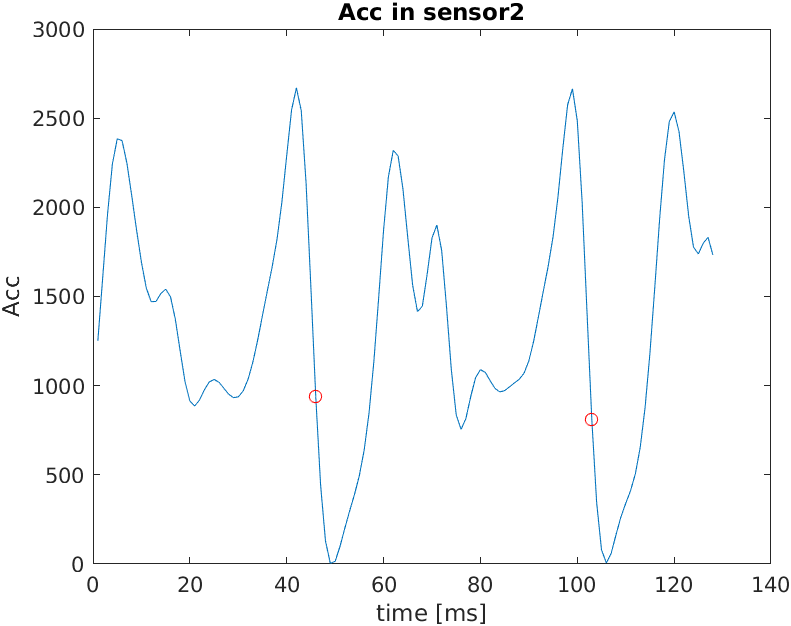
\includegraphics[width=\textwidth]{acc_step_s1_p2}
		\caption{acceleration of walking in y axis of ankle sensor}
		\label{fig:three sin x}
	\end{subfigure}
	\hfill
	
	
	\begin{subfigure}[b]{1\textwidth}
		\centering
		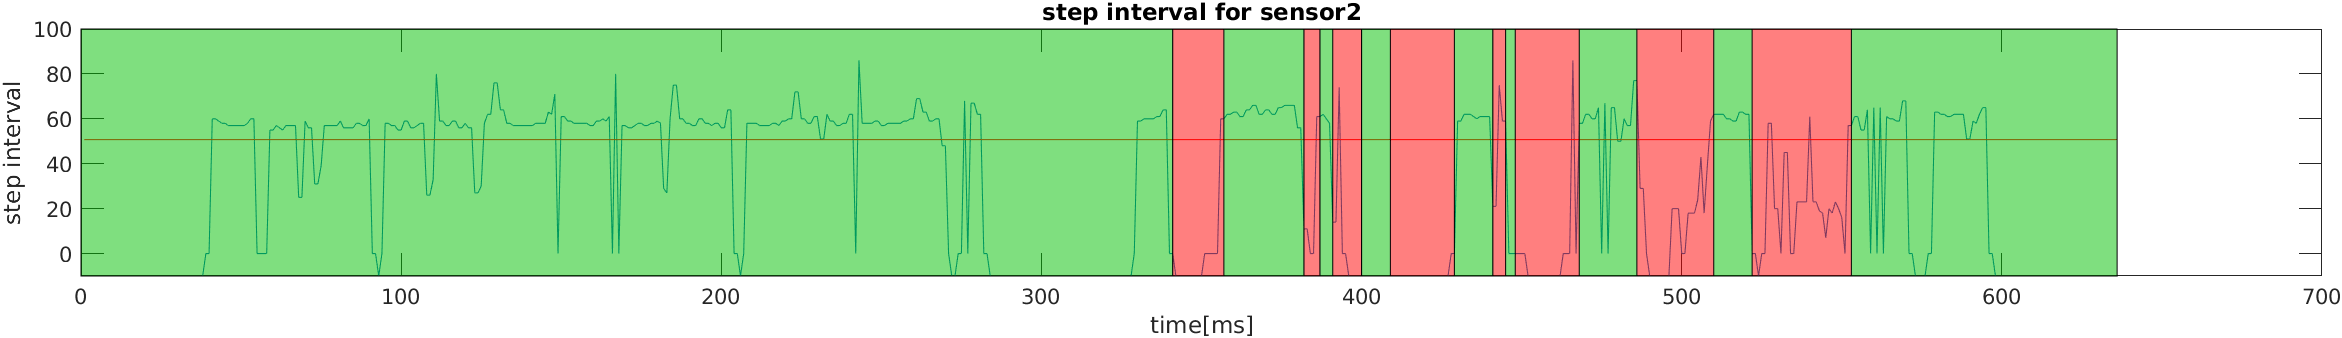
\includegraphics[width=\textwidth]{step_interval_fast_s2_p2}
		\caption{measured step interval}
		\label{fig:five over x}
	\end{subfigure}
	
	
	
	\caption{The red area shows FoG, the green area shows non-FoG(a)The acceleration in y axis of ankle sensor, the purple part shows stop, the blue part shows normal walking.(b)Zoom into one of the walking window, two U shape can be observed, the red point shows the detected step.(c)The time interval between two detected points shows where the FoG might be}
	\label{fig:three graphs}
\end{figure*}

	


% Feature selection
% Features Extraction
\begin{center}
	\subsection{FeatureSelection}
\end{center}

After the features are extracted, generally we can just feed them into a dimension reduction tool like LDA. However, the result of using features directly does not generate good results.

In a larger scale, for some patient, certain features are more effective to detect FoG than the others. This can be explained with the fact that different patients have different symptoms during the FoG, according to the research of (Freezing-of-Gait Detection Using Wearable-Sensor Technology and Neural-Network Classifier
Author: Parisa Tahafchi, Jack Judy). FoG can be shown as festination, akinesia and trembling.

According to the observation, different gait features have different dependencies with labeled data. Also, different patients have different gait features during the FoG, therefore, it is important to find out which features are more efficient for each patient. Although LDA is capable of selecting not meaningful features out by giving them very small weights, but this ability is fully depend on the quality of data set.

We selected filter method to do feature selection, because it selects features independently for any machine learning algorithm. It can help us remove features that contains little information.

Correlation filter method such as Spearman's rank correlation can be used to measure the degree of association between two set of variables with a monotonic function. It is capable of handling non-linear functions in compare with Pearson correlation.

Statistical method such as mutual information a measure of the mutual dependence of two variables. It measures the amount of information obtained about one variable through observing the other variable. 

In the experiment we are going to use both of them and make comparison.

% Feature thresholding
\begin{center}
	\subsection{Thresholds and feature reduction}
\end{center}

To solve the unbalanced data problem, it is necessary to do cleaning to dataset before processing it. According to the measurement of Baechlin et al, when the patient is standing still, its energy between [0-8Hz] frequency band is significantly lower than other status. Therefore, we can first exploit such characteristic and filter out windows when patient is standing and only make classification between FoG and walking or turning. It is also possible to try other features as thresholds, however, we need to make sure that the filtered region is not broken into small pieces so that the time continuity around FoG is still valid, this guarantees an evaluation standard that we are going to talk about in the next part.

After we get the cleaned dataset and selected features, we are ready for LDA. Since simple thresholds on all these features is still too complicate and computational expensive. We still need this step to further reduce the dimension down to a level which is easier for classification.

The output dimension of LDA is depends on classification method. Higher dimension comes with higher performance at the cost of more computation and memory resource requirement.

The simplest version of classifier is dealing with one dimensional features. In such case, the classifier only need to draw a line and discriminate the data based on this threshold. The last step is to design a classifier which gives us this line. It is worth noted that the design of classifier is closely coupled with evaluation standard, which need to be clarified first.


% Evaluation standard
\begin{center}
\subsection{Classification and Evaluation standard}
\end{center}


	Most papers regarding the FoG detection uses classical classification quality metrics,such as precision, specificity Recall and F1-Score.
	
	However, such classification standard does not consider the user experience and time continuity.
	
    Since the objective is to detect FoG in a realtime way, it is desired that the time window before the actual FoG is also classified as a FoG. Therefore, the FoG period is extended into a a larger scale.
    
    Considering that a false alarm happens just after  the FoG is not so annoying as a false alarm during a normal walk, we also consider it as a correct label.
    
    Also, we make an assumption that the patient can recover from the FoG as long as he get an alarm for a certain time.
    
    In conclusion, the following situations need to be reconsidered:

    \begin{enumerate}
    	\item The FoG rising edge: If one continuous window sequence before the rising edge is classified as a FoG period, then the whole window sequence is considered as correct labeled even part of them are not labeled as FoG in the dataset.
    	
		\item During the FoG period: If the edge is detected and solved with one filter window, we consider that the patient would have stop experiencing the FoG period, therefore, the whole continuous FoG period is considered as solved.  Otherwise, if the FoG is detected after the coming edge, only part of the FoG period is considered as solved
		
		\item Whenever one FoG period ends, if one continuous window sequence is correct labeled at this point, then all filter window continuously followed are considered as correct.		
    \end{enumerate}

	In summary, such evaluation standard punishes the wrong results that near correct result less in compare with original evaluation standard. It focuses on how to make the false alarm less annoying and at the same time covering more FoG. 

	In this way, we have a new evaluation standard. New Precision stands for the percentage of correct alarm in all windows labeled as FoG, which is similar to Precision. New Recall stands for how many FoG windows are solved, which is the similar as recall before.
	
	\begin{equation}
	\mathbf{New Precision} = \frac{\sum corrcect FoG alarms}{\sum all FoG alrams}
	\end{equation}
	
	\begin{equation}
	\mathbf{New Recall} = \frac{\sum solved FoG}{\sum all FoGs exists}
	\end{equation}
	
	\begin{equation}
	\mathbf{New F1-Score} = 2*\frac{NewPrecision * NewRecall}{NewPrecision+NewRecall}
	\end{equation}
	
	
	To find a separating line, we employ the same method as in decision tree. Several possible value between the mean of FoG features and non-FoG features is going to be selected, then the quality metrics is going to be calculated. 
	
	\begin{figure}		
	\begin{subfigure}[b]{0.45\textwidth}
		\centering
		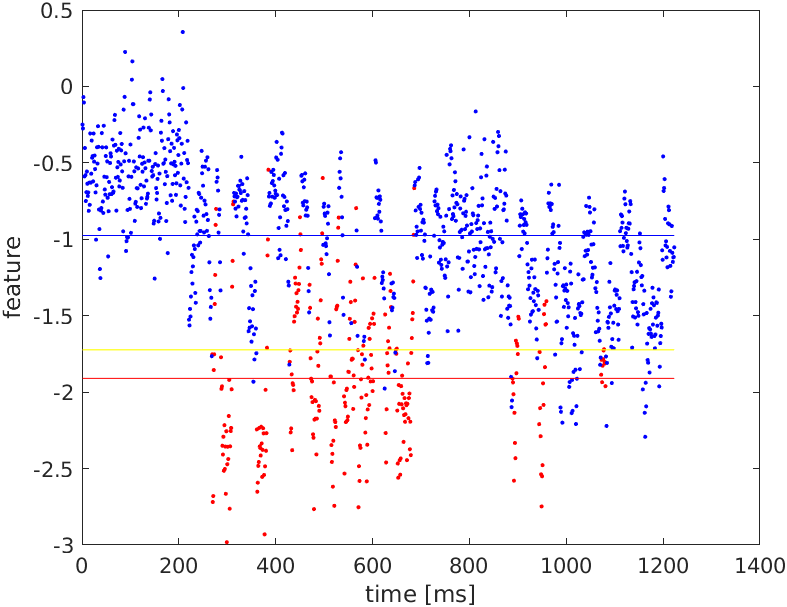
\includegraphics[width=\textwidth]{classifier}
		\caption{lda feature reduced to one dimension}
		\label{fig:y equals x}
	\end{subfigure}
	\caption{The blue line shows the mean value of features in non-FoG windows, the red line shows the mean value of features in FoG windows. The target is to find a separating line(yellow) which best discriminate the data}
	\label{fig:three graphs}
	\end{figure}
\begin{figure}		
	\centering
	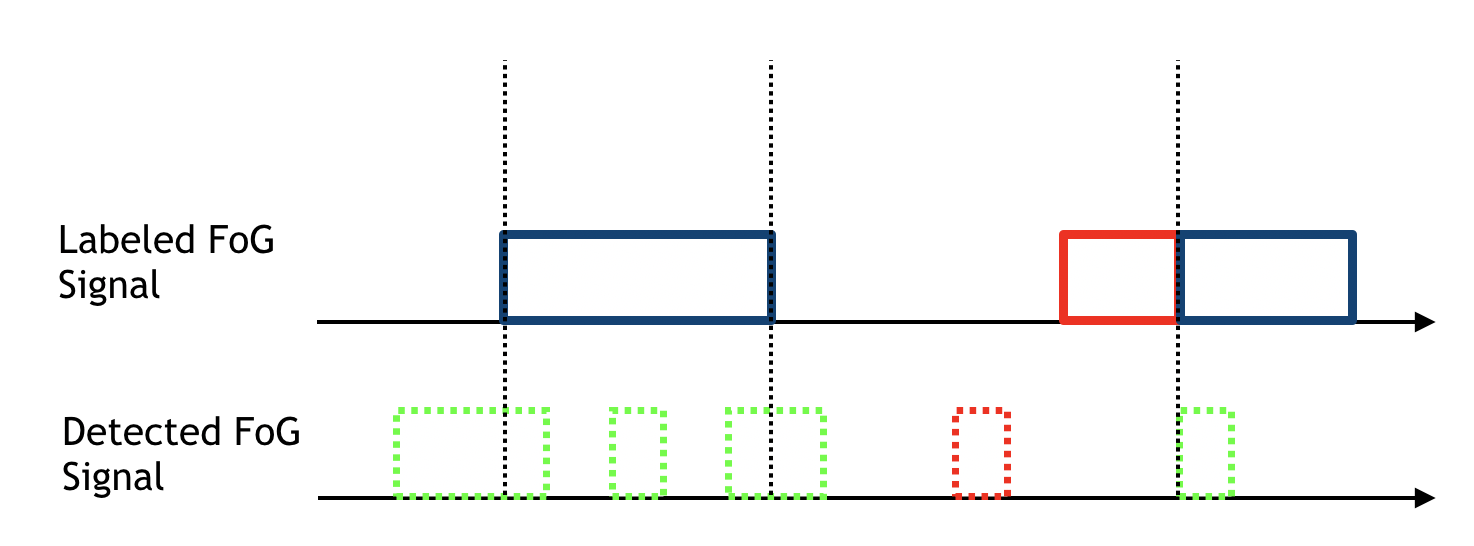
\includegraphics[width=0.45\textwidth]{evaluation}
	\caption{Evaluation method}
	\label{fig:y equals x}	
\end{figure}
	In decision tree algorithm, generally gini index is going to be used, However, it does not performs so well with unbalanced data since the line is always too agressive with high Recall and low precision. So we tried to use a  scaled version of gini index in which we make each FoG points n times bigger in terms of number, n is the ratio of number between the non-FoG points and FoG points.
	
	Also we can use the new evaluation standard and try to find a best result with highest F1-score.
	

	
% Classifier design
\section{Result}
    
	The first result worth mentioned is feature selection.
    After the feature extraction, we calculate mean value Spearman rank correlation and mutual information of each feature value and labels for all patients, the result is shown in the Figure 3. 
    
    The result of two methods generally coincide with each other. The three sensors placed in different locations and three axes can been seen as nine channels. From picture a and b, it is clear that channel1(Horizontal forward acceleration on ankle), channel 2 (Vertical acceleration on ankle) and channel 5 (Vertical acceleration above knee) have the highest dependency with FoG symptoms. On the other hand, picture c and d shows the dominant frequency, locomotion energy and freezing index has the closest relationship with FoG among all features.
    
    According to the observation, since cross correlation and wavelet mean have quite low score and at the same time  they are quite expensive in terms of computation, we decide to throw them from the list of features.
    
    
   	\begin{figure*}
    	
    	\begin{subfigure}[b]{0.47\textwidth}
    		\centering
    		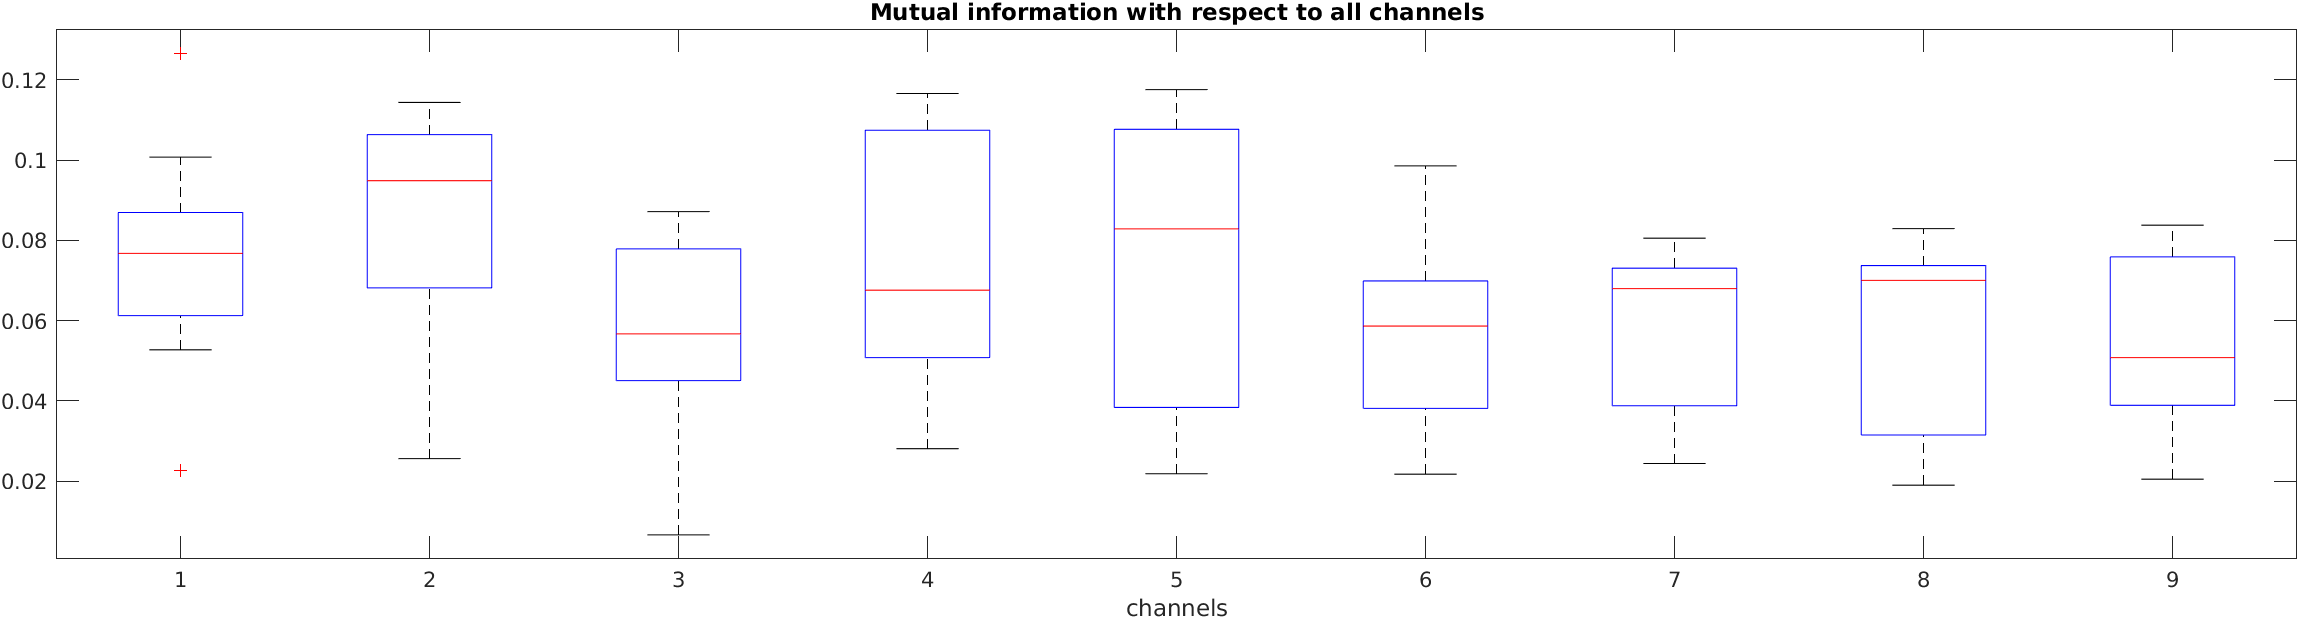
\includegraphics[width=\textwidth]{MutualA}
    		\caption{}
    		\label{fig:y equals x}
    	\end{subfigure}
		\hfill
    	\begin{subfigure}[b]{0.47\textwidth}
		\centering
		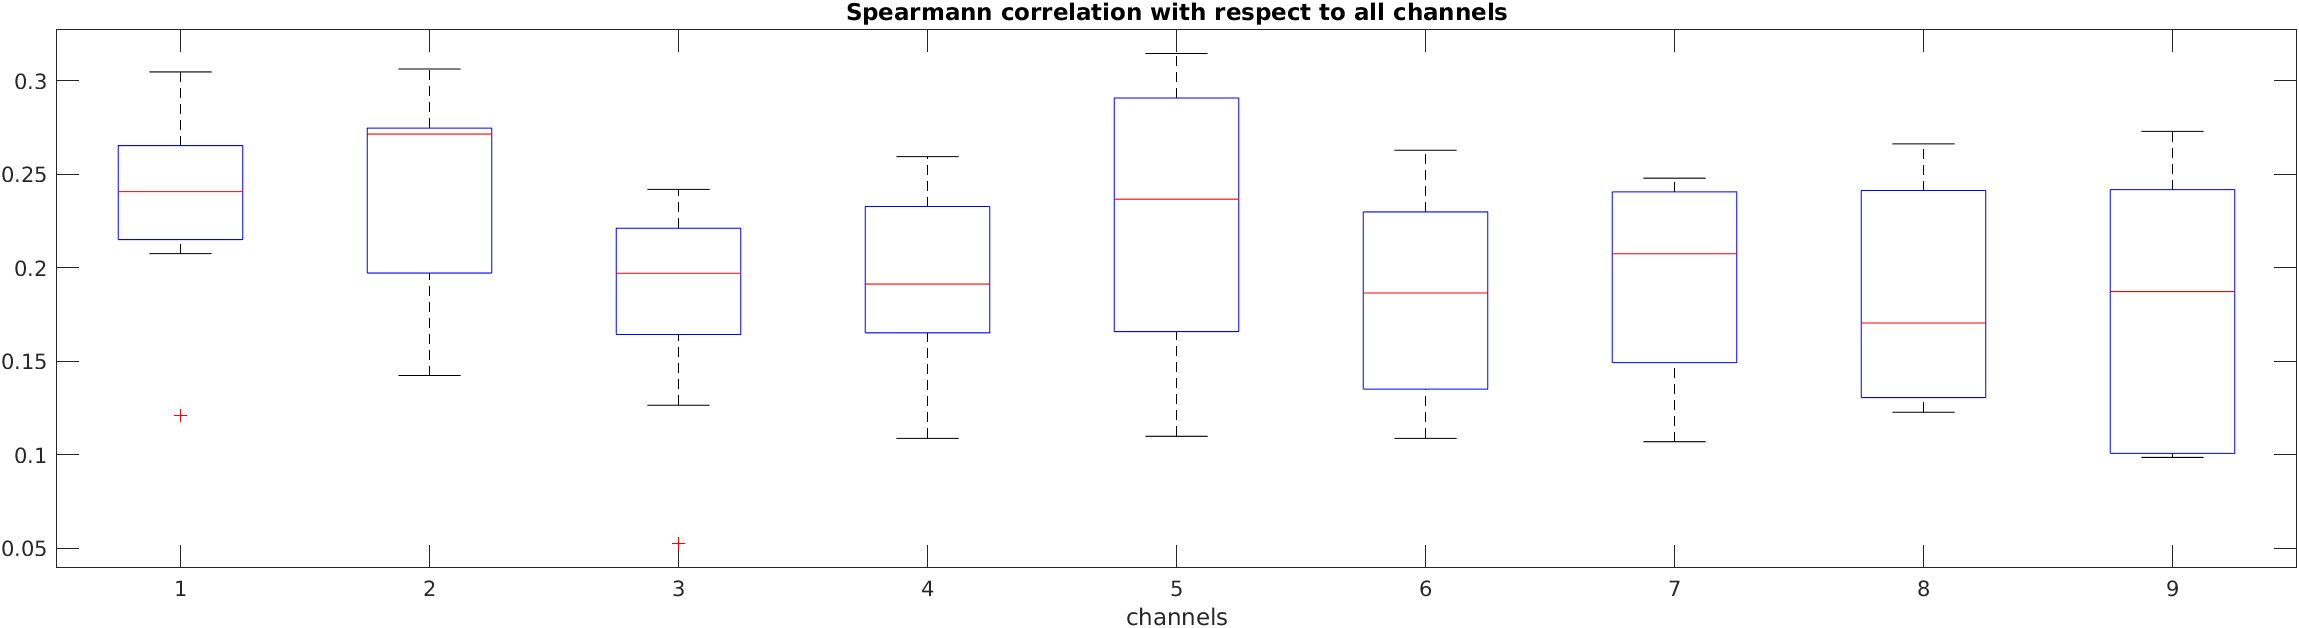
\includegraphics[width=\textwidth]{spearmannA}
		\caption{}
		\label{fig:y equals x}
		\end{subfigure}
	
		\begin{subfigure}[b]{0.47\textwidth}
			\centering
			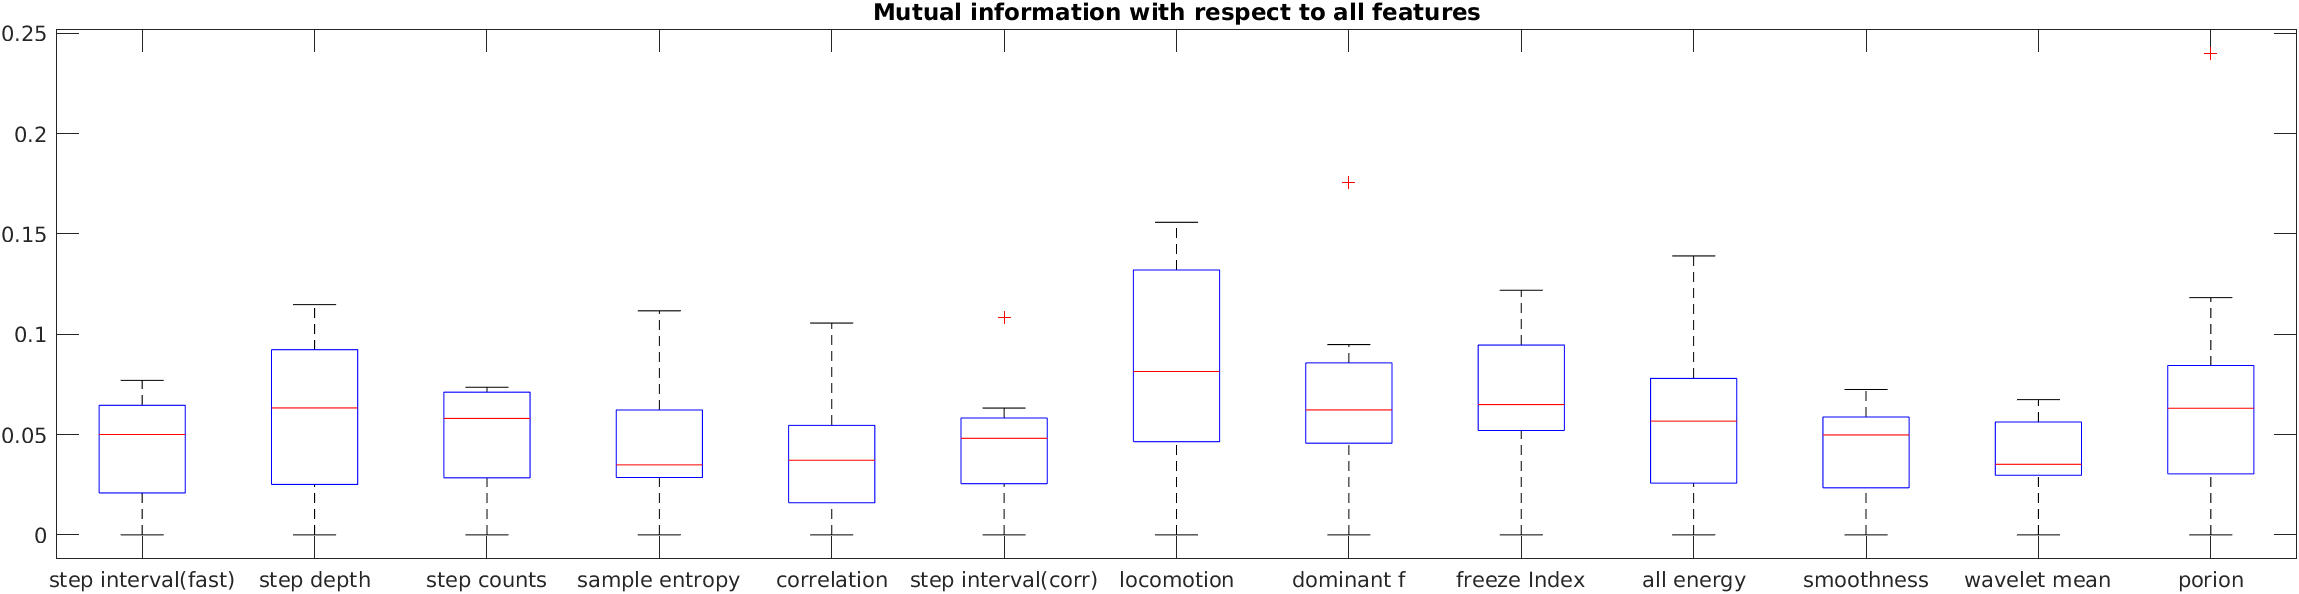
\includegraphics[width=\textwidth]{MutualF}
			\caption{}
			\label{fig:y equals x}
		\end{subfigure}
		\hfill
		\begin{subfigure}[b]{0.47\textwidth}
			\centering
			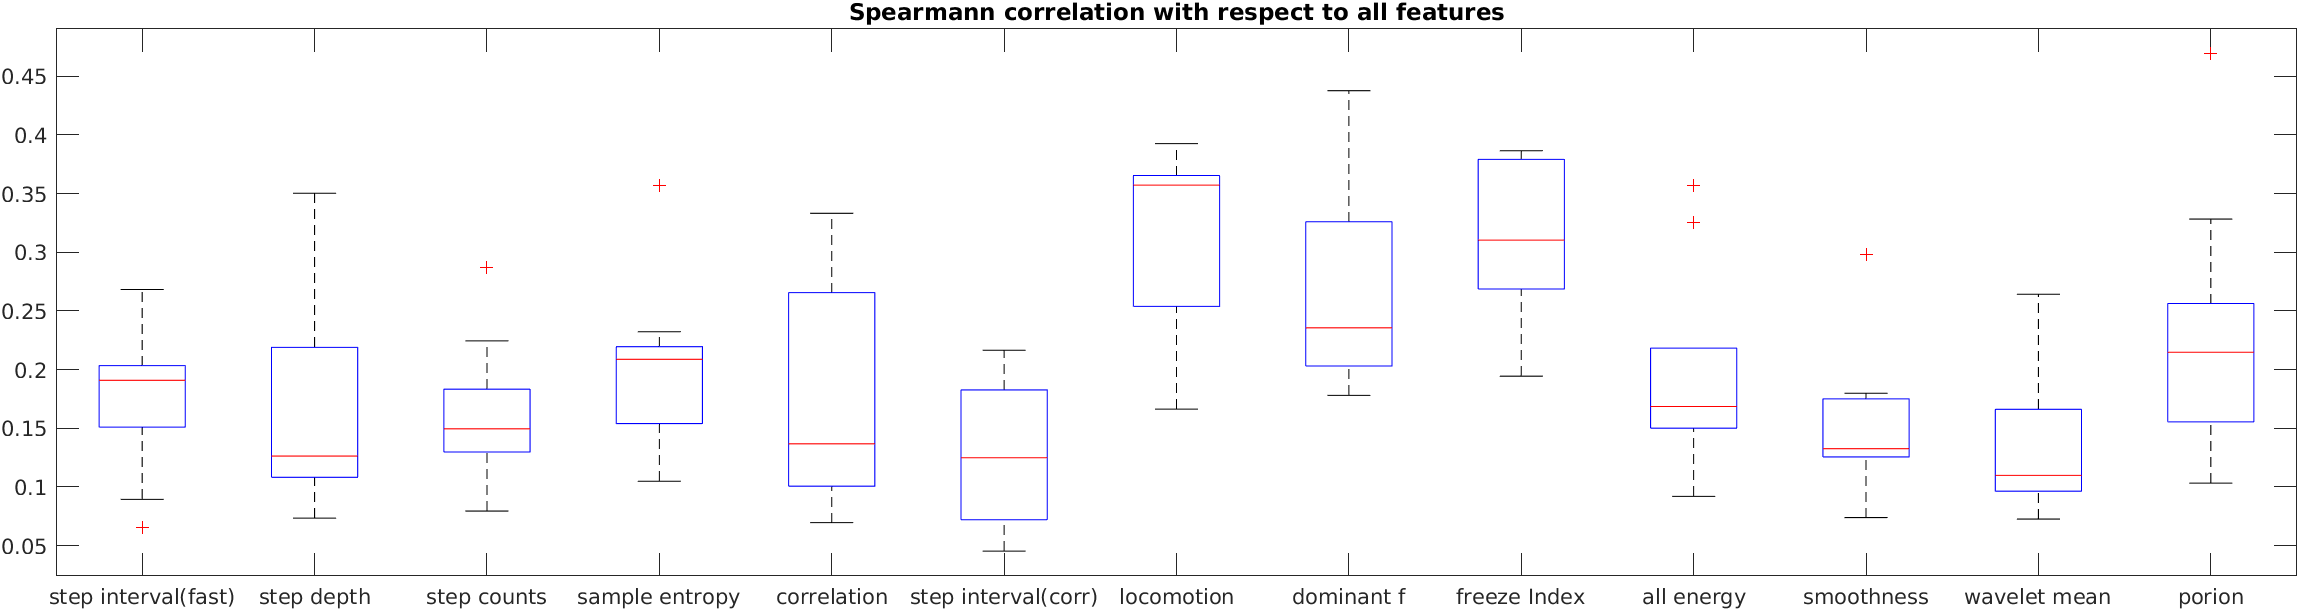
\includegraphics[width=\textwidth]{spearmannF}
			\caption{}
			\label{fig:y equals x}
		\end{subfigure}
    
    	\caption{Figure(a) shows the mutual information between channels and FoG;Figure(b) shows the Spearmann correlation between channels and FoG;
    	Figure(c) shows the mutual information between features and FoG;
		Figure(d) shows the Spearmann correlation between features and FoG;}
    	\label{fig:three graphs}
    \end{figure*}
    
The result using new evaluation methods is shown in Table 1,2 and 3. It is easy to find that our method performs better than the method proposed by Bachelin in all cases except patient with ID 5. 



 \begin{table*}
    \begin{center}
   		\begin{tabular}{  |p{0.5cm}||p{1.3cm}|p{1.3cm}|p{1.3cm}|p{1.3cm}|p{1.3cm}|p{1.3cm}|p{1.3cm}|p{1.3cm}|p{1.3cm}| }
		\hline
		\multicolumn{4}{|c|}{Result with Spearman's correlation} &\multicolumn{3}{|c|}{Result with Mutual information}&\multicolumn{3}{|c|}{Result with Bachelin's method}  \\
	
		\hline
		 ID &  precision &  recall &  F1-score &  precision &  recall &  F1-score &  precision &  recall &  F1-score\\
		\hline
		1 & 0.8606 &0.8419 & 0.8511 & 0.7808 &0.8972 & 0.8350 & 0.6685 &0.7470 & 0.7056 \\
		2 & 0.8854 &0.9315 & 0.9079 & 0.9286 &0.8191 & 0.8704  & 0.7228 &0.8142 & 0.7658\\ 
		
		3 & 0.8478 &0.9733 & 0.9062 & 0.8357 &0.9793 & 0.9018 & 0.8050 &0.9111 & 0.8548 \\   
		
		5 & 0.7524 &0.7750 & 0.7635  & 0.7372 &0.8091 & 0.7682  & 0.8161 &0.8269 & 0.8214 \\
		
		6 & 0.7338 &0.9152 & 0.8145 & 0.8232 &0.8799 & 0.8506 & 0.5471 &0.8763 & 0.6736 \\
		
		7 & 0.7704 &0.7773 & 0.7738 & 0.7260 &0.8389 & 0.7783&  0.7184 &0.6066 & 0.6578\\
		
		8 & 0.8591 &0.8861 & 0.8772 & 0.8286 &0.8545 & 0.8413 & 0.7738 &0.8176 & 0.7951   \\	
		
		9 & 0.7302 &0.8916 & 0.8028 & 0.9013 &0.6054 & 0.7243 & 0.7294 &0.7504 & 0.7398\\
		\hline
		\end{tabular}
	\caption{detection result}
\end{center}
     \end{table*}
   If we look close to the result of detection in figure. The left figure shows the original method, and the right figure shows the result with new detector, it is clear than the number of false alarm decreases.
   
   
    \lipsum[1]
 
    
    \begin{figure}
    \begin{center}
    	
    	\begin{subfigure}[b]{0.45\textwidth}
    		\centering
    		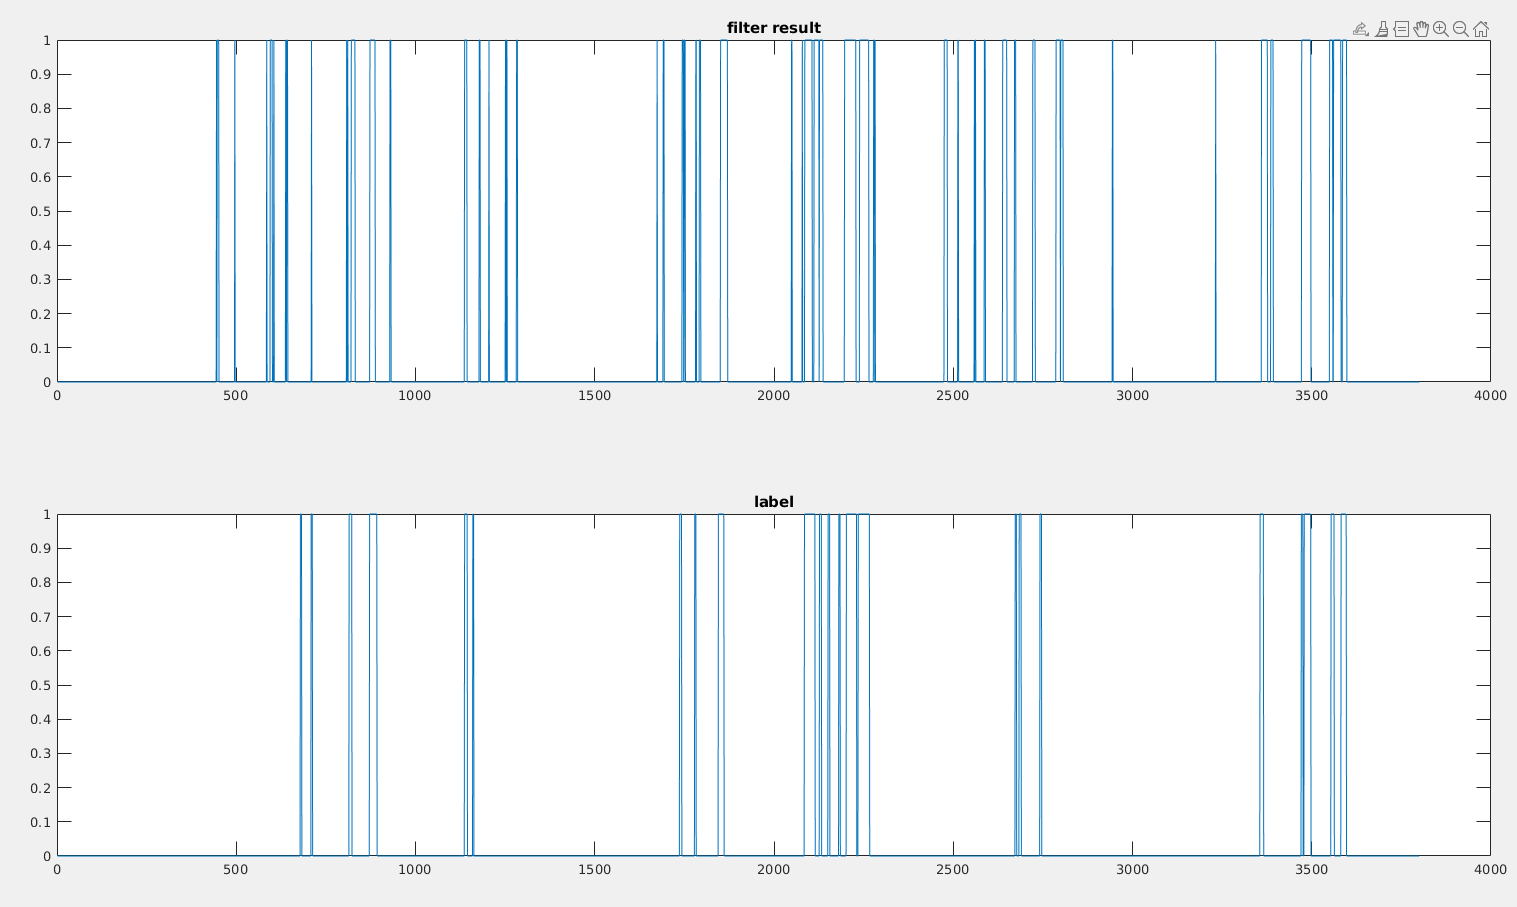
\includegraphics[width=\textwidth]{method1}
    		\caption{}
    		\label{fig:y equals x}
    	\end{subfigure}
    	\hfill
    	\begin{subfigure}[b]{0.45\textwidth}
    		\centering
    		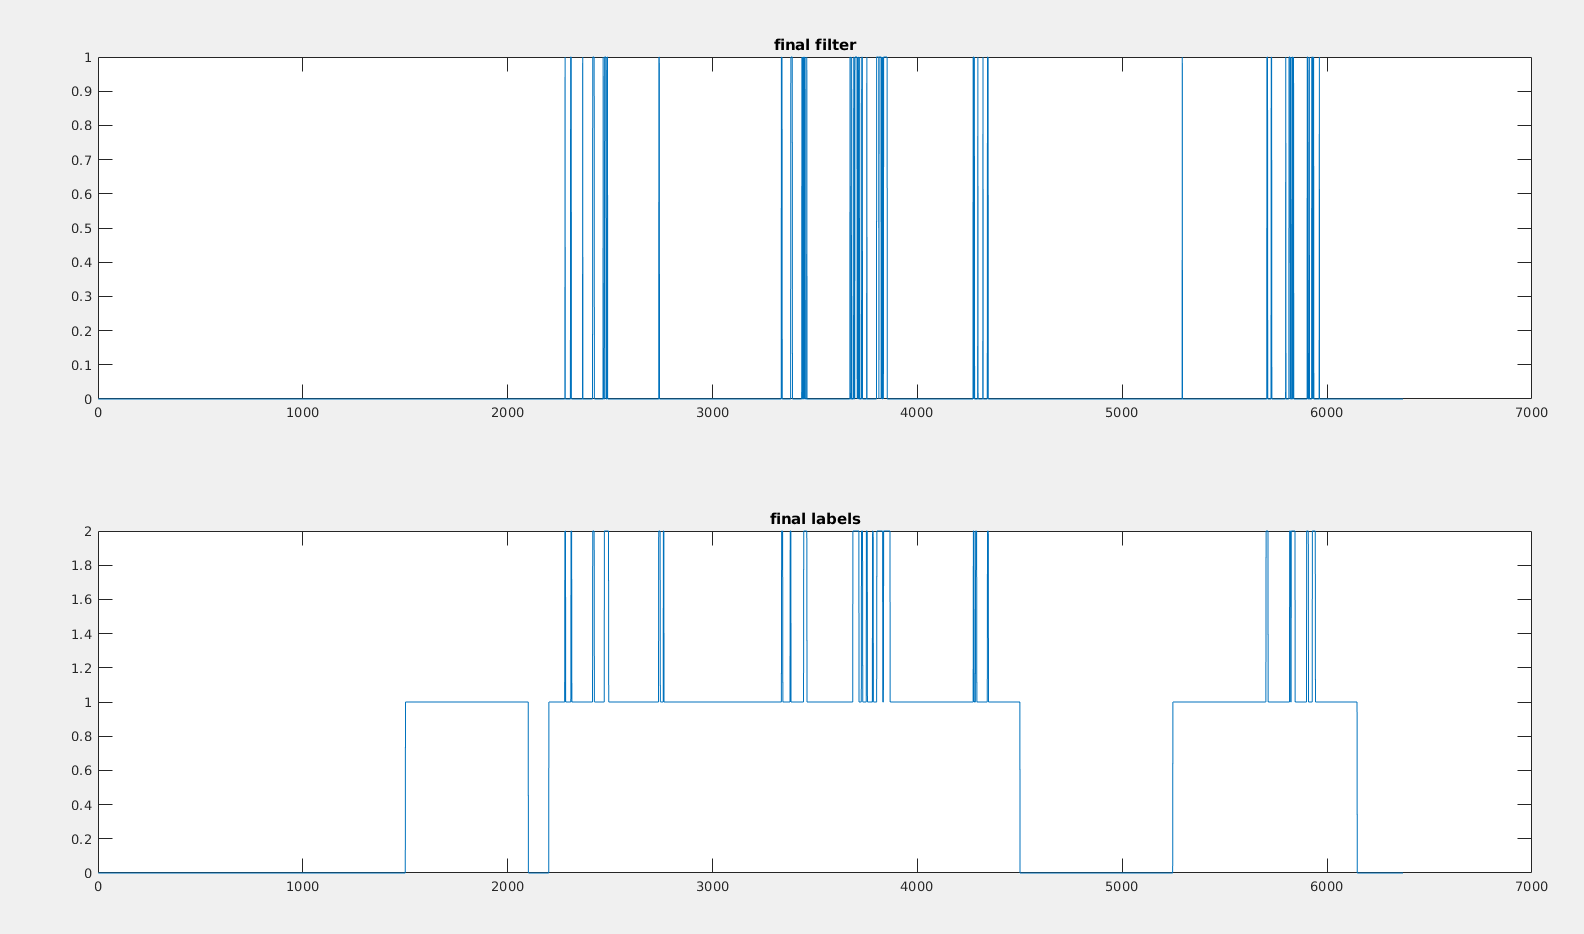
\includegraphics[width=\textwidth]{method2}
    		\caption{}
    		\label{fig:y equals x}
    	\end{subfigure}
    	
    	
    	
    	\caption{Figure(a) shows the mutual information between channels and FoG;Figure(b) shows the Spearmann correlation between channels and FoG;
    		Figure(c) shows the mutual information between features and FoG;
    		Figure(d) shows the Spearmann correlation between features and FoG;}
    	\label{fig:three graphs}
 \end{center}	
   
 \end{figure}
    


% Hardware design
\section{Implementation}
   The implementation is mainly divided into three part: Graphic user interface implemented with Qt, data training written in python and C code that running on the hardware. Since we don't have sensors that does the measurement, UART is applied to send data in window form (128*9 integer) to the hardware.      
   
   In the graphic user interface, we can choose the auto mode which uses the method mentioned before to select features, or we can manually configure the sensors numbers and lda features. The manual configuration mode is available since expert can select features that meaningful for each person individually, it may outperform the auto method which is based on data. Besides, for both mode we can also select classifiers and thresholds and relevant parameters. 
   
   After the configuration part is done, relevant data will be feed into python code as parameters and training process starts. After the training process is finished, it returns and informs the user and save results into a file at the same time. 
   
   Then user can further use GUI to send results of training and raw data measurement in window form to hardware with UART, the hardware returns the detection result back to user interface before it receives new window.
   
   The hardware we used here is the nRF52 Development kit which has 512 kB flash and 64 kB RAM memory space.  
   
   
  
% Conclusion and futhure work
\section{Conclusion}
\lipsum[1]
\lipsum[1]
    

\bibliographystyle{ieeetr}
\bibliography{other/bibliography}
\nocite{*}
		
\end{document}